% ===========================================================================
\section{Extension: RECFAST recombination}\label{sec:recfast}
% ===========================================================================

The Peebles model of Sec.~\ref{sec:m2} treats hydrogen as a three-level atom with the case-B rate of
Ref.~\cite{Callin2006}, and helium in Saha equilibrium. In the comparison with CLASS (Sec.~\ref{sec:validation}) this
left differences of up to 1\% in TT and 3\% in EE, mostly through the damping tail and the width of the visibility
function. The code now uses RECFAST~\cite{Seager1999,Wong2008,RubinoMartin2010} by default (the default of CAMB, and of CLASS before
version~3), which reproduces the multi-level calculations to $\sim0.1\%$ in $X_e$ with three
ordinary differential equations. The Peebles model is kept as an option (\texttt{recombination = peebles}) and is
used for Secs.~\ref{sec:m2}--\ref{sec:m4}.

\subsection{Equations}

RECFAST evolves the hydrogen ionization fraction $x_{\rm H}=n_{\rm HII}/n_{\rm H}$, the singly ionized helium
fraction $x_{\rm He}=n_{\rm HeII}/n_{\rm He}$ and the baryon temperature $T_b$, with $X_e=x_{\rm H}+f_{\rm He}x_{\rm He}$
and $f_{\rm He}=Y_p/[3.9715(1-Y_p)]$ (the helium-to-hydrogen mass ratio is 3.9715, not 4 as in Sec.~\ref{sec:m2}).
For hydrogen,
\begin{align}
\frac{dx_{\rm H}}{dz}&=\frac{X_ex_{\rm H}n_{\rm H}\alpha_{\rm H}-\beta_{\rm H}(1-x_{\rm H})e^{-h\nu_{\rm Ly\alpha}/k_BT_b}}
{H(1+z)}\,C_{\rm H},\\
C_{\rm H}&=\frac{1+K_{\rm H}\Lambda_{2s1s}n_{1s}}{F_{\rm H}^{-1}\big(1+K_{\rm H}\Lambda_{2s1s}n_{1s}\big)+K_{\rm H}\beta_{\rm H}n_{1s}},
\end{align}
with $n_{1s}=n_{\rm H}(1-x_{\rm H})$. The case-B recombination coefficient is the fit
$\alpha_{\rm H}=10^{-19}\,a\,t^b/(1+c\,t^d)\,{\rm m^3\,s^{-1}}$, $t=T_b/10^4$\,K, of
Ref.~\cite{Pequignot1991}, and $\beta_{\rm H}=\alpha_{\rm H}(2\pi m_ek_BT_b/h^2)^{3/2}e^{-h\nu_{2s}/k_BT_b}$ is the
photoionization rate from $n=2$. The Peebles factor $C_{\rm H}$ is the probability that an atom in $n=2$ reaches
the ground state before it is ionized: through the two-photon decay ($\Lambda_{2s1s}=8.22\,{\rm s^{-1}}$) or
through the redshifting of Lyman-$\alpha$ photons out of the line, with
\begin{equation}
K_{\rm H}=\frac{\lambda_{\rm Ly\alpha}^3}{8\pi H}\Big[1+\sum_{i=1}^2A_ie^{-[(\ln(1+z)-z_i)/w_i]^2}\Big].
\end{equation}
The two Gaussians in $\ln(1+z)$ (RECFAST 1.5) and the fudge factor $F_{\rm H}=1.125$ (1.14 in earlier versions)
calibrate the three-level atom against the multi-level calculations of Refs.~\cite{RubinoMartin2010,Wong2008}: they
absorb the effects of the high-$n$ states, of the two-photon transitions from higher levels and of the Lyman series
feedback. For neutral helium RECFAST uses the same form for the He\,I singlet system (2$^1$S two-photon rate
$51.3\,{\rm s^{-1}}$, the fit of Ref.~\cite{Verner1996} for the recombination rate), with two additions that make
helium recombine much faster than Saha-equilibrium hydrogen-like treatments: the escape of the 2$^1$P photons is
helped by their absorption by the small amount of neutral hydrogen present at $z\sim2000$ (a continuum-opacity term
calibrated by the fudge $F_{\rm He}=0.86$), and atoms can also recombine through the triplet 2$^3$P state. The
baryon temperature follows Compton heating by the CMB and adiabatic cooling, as before.

\subsection{Implementation}

As in RECFAST, the solution has three phases. While both hydrogen and helium are close to equilibrium we use the
Saha equations of Sec.~\ref{sec:m2}, now for H$^+$, He$^+$ and He$^{++}$ together. When the singly ionized helium
fraction drops below 0.995 ($z\approx2900$) we integrate the helium equation, with hydrogen still in Saha
equilibrium, and when $x_{\rm H}<0.995$ ($z\approx1600$) we integrate the full system $(x_{\rm H},x_{\rm He},T_b)$.
The equations are stiff, because the rates exceed $H$ by many orders of magnitude when the gas is close to
equilibrium, and we use an implicit BDF method. The constants (energy levels from the measured inverse wavelengths,
Einstein coefficients, fitting formulae) are those of RECFAST 1.5 as used in CLASS. The switch to the full hydrogen
equation leaves a small kink in $dX_e/dx$ at $z\approx1600$, where the visibility function is negligible
($10^{-13}$ of its maximum); elsewhere $\tau''$ agrees with a finite difference of $\tau'$ to a few $10^{-6}$. The whole calculation takes
0.35\,s.

\subsection{Validation}

Figure~\ref{fig:recfast} compares $X_e$ without reionization and the unlensed spectra with CLASS run with RECFAST.
\begin{itemize}
\item $X_e$ agrees with CLASS RECFAST to $3.3\times10^{-4}$ for $0\le z\le8000$, including
      both helium recombinations (the largest difference is at $z\approx1530$, just after the switch to the full hydrogen equation); the Peebles model differs by up to 3.8\%
      during hydrogen recombination ($800<z<1600$). Last scattering is at $z_*=1089.79$
      (CLASS: 1089.79) with $r_s(z_*)=144.421\Mpc$ (CLASS: 144.421).
      The difference from HyRec, CLASS's default, is up to 1\% during
      helium recombination and in the freeze-out tail, and 0.11\% during
      hydrogen recombination.
\item The rms difference of TT from CLASS RECFAST is 0.048\% for
      $30\le\ell\le1000$ and 0.29\% for $1000<\ell\le2000$, against
      0.64\% and 0.75\% with the Peebles
      model. For EE the rms difference is 0.32\% and
      0.46\%, against 1.4\% and
      1.4\%. The largest single-$\ell$ EE differences,
      2.3\% for $\ell\le30$, are at the zeros of the reionization feature.
\item In CLASS, the RECFAST and HyRec spectra differ by less than $10^{-3}$ rms (dashed in Fig.~\ref{fig:recfast}).
      Our remaining differences from CLASS, which grow to a few $10^{-3}$ in the damping tail, are larger than this.
      They therefore come from other numerical approximations in the code, and recombination is no longer the
      limiting approximation.
\end{itemize}

\begin{figure*}
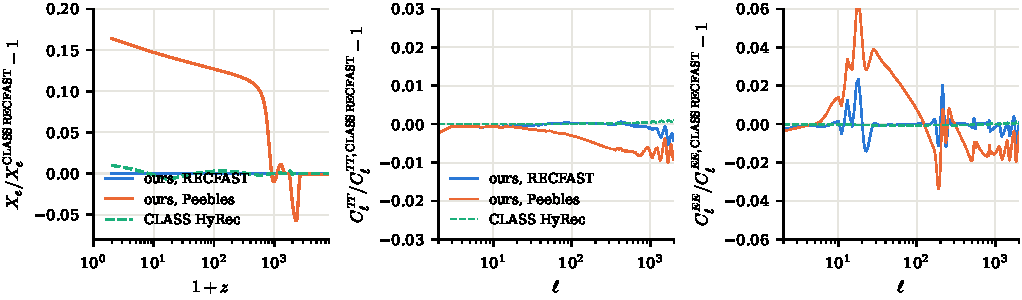
\includegraphics[width=\textwidth]{recfast}
\caption{The RECFAST recombination model. \emph{Left:} $X_e(z)$ without reionization relative to CLASS run with
RECFAST, for our RECFAST (blue) and Peebles (orange) models; the dashed line is CLASS with HyRec. \emph{Middle,
right:} the unlensed TT and EE spectra (with reionization) relative to CLASS RECFAST.}
\label{fig:recfast}
\end{figure*}
